\subsection{Weak Scaling Study}
\label{subsec:weak-scaling-study}

The weak scaling study evaluates the performance of the ray tracing implementation as the problem size, measured by scene complexity, increases. This experiment measures runtime and speedup for scene complexities ranging from 1 to 64 and thread counts of 1, 2, 4, 8, 16, 32, 64, 128, and 256. Dynamic scheduling with a chunk size of 1 was used for all configurations.

The results indicate that more complex scenes benefited significantly from parallelization. For example, at a scene complexity of 1, the maximum speedup achieved was only 1.3 times using 256 threads. In contrast, a scene complexity of 64 achieved a speedup of 77.5 times with 256 threads. This highlights the significant impact of scene complexity on the efficiency of parallel execution. As shown in Figure~\ref{fig:scene-complexity-speedup}, scaling performance improves with increasing scene complexity; however, the performance gains plateau as scene complexity reaches 64.

The performance plateau at higher scene complexities suggests potential bottlenecks such as synchronization overhead, memory contention, or limitations inherent to the computational platform. These findings emphasize the importance of optimizing workload distribution and employing larger problem sizes to better utilize parallel resources. Further investigation is required to determine the exact causes of the performance plateau, which could include analyzing memory access patterns, thread synchronization mechanisms, or identifying architectural constraints. Additional details on memory usage inefficiencies and their impact on scaling behavior are discussed in Appendix~\ref{sec:memory-footprint}.

\begin{figure}
    \centering
    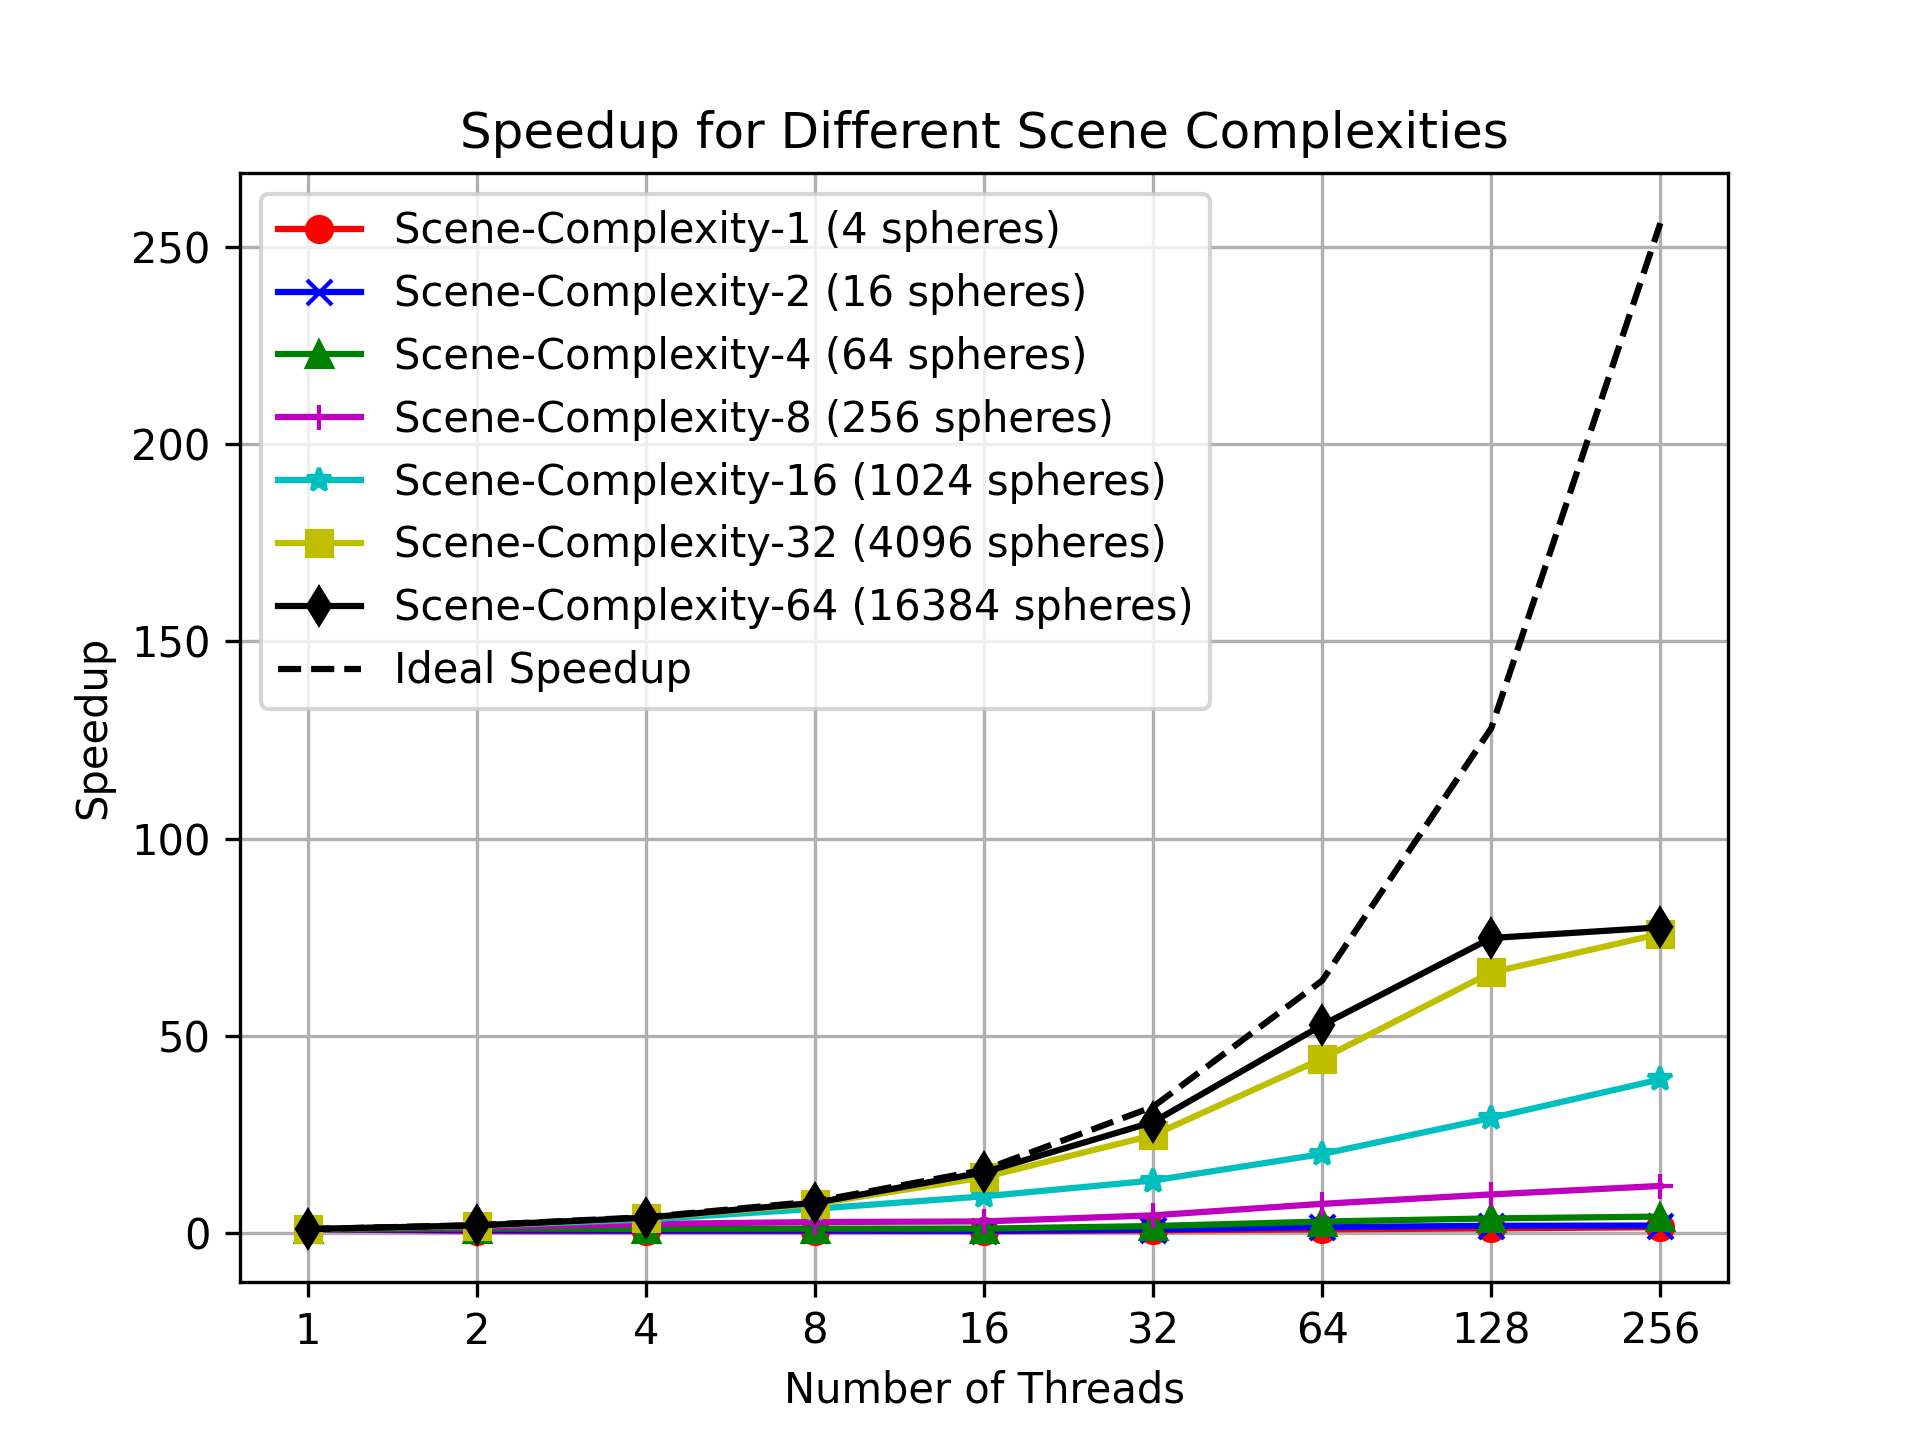
\includegraphics[width=1.0\linewidth]{images/scene_complexity_speedup_comparison.png}
    \caption{Speedup achieved for varying scene complexities under dynamic scheduling. The results demonstrate improved scaling for higher complexities, but with diminishing returns as complexity increases.}
    \label{fig:scene-complexity-speedup}
\end{figure}
\FloatBarrier